\chapter{Proposed Method}
\label{chapter:proposed-method}

This Chapter describes each of the modules that integrate the method used to
create the trading strategy proposed in this work and how their integration is
performed.

\section{Preprocessing a Financial Market using Retracements}
\label{section:preprocessing-a-financial-market-using-retracements}

Many works that propose methods for financial market forecasting or modelling do
not preprocess the time series that represent a financial market \cite{}. As a
consequent, some of the models that try to simulate these markets have an
additional complexity layer to deal with, similarly to the difficulty that a
neural network would encounter at trying to do facial recognition to
un-processed images. For this reason, a facial recognition algorithm needs to be
fed images that have been rotated, scaled down, and reduced in noise by using
image processing algorithms \cite{}. After doing this preprocessing, it is
easier for a modelling algorithm to create a model of a financial market, as it
does not have to waste time and effort at trying to distinguish between noise
and significant data.

For financial market preprocessing, an option is to use technical indicators:
mathematical calculations that are applied to time series that represent the
historical prices of a financial market. As an example of a technical
indicator's use, a moving average -- a series of averages of different subsets
of the full data set -- can remove the noise in a market by creating a smooth
line that represents each of the data points in the time series, as can be seen
in Figure \ref{figure:moving-average-noise}. Other technical indicators can
provide other types of insight about a market, such as the market's volatility,
support and resistance levels, and overbought and oversold levels, among others
\cite{}.

\begin{figure}
\caption{Using a moving average to remove the noise from a financial market time
series} \centering
\includegraphics[width=1.0\textwidth]{img/moving-average-noise.png}
\label{figure:moving-average-noise}
\end{figure}

This thesis emphasizes that a financial market's data should always be
preprocessed, and for this reason the proposed method makes this a
requirement. Although any preprocessing method could be used with the proposed
method, with minimal modifications to the other modules conforming the method, a
preprocessing method that yields multiple insights about the market is
preferred. Additionally, these insights should be numerically represented,
should be continuous and their possible values should encompass an interval. For
example, multiple technical indicators can be used to provide different kinds of
insights. Figure \ref{figure:multiple-technical-indicators} shows how three moving
averages can be used to represent different perspectives of the market.

\begin{figure}
\caption{Using three moving averages to represent different perspectives of the market} \centering
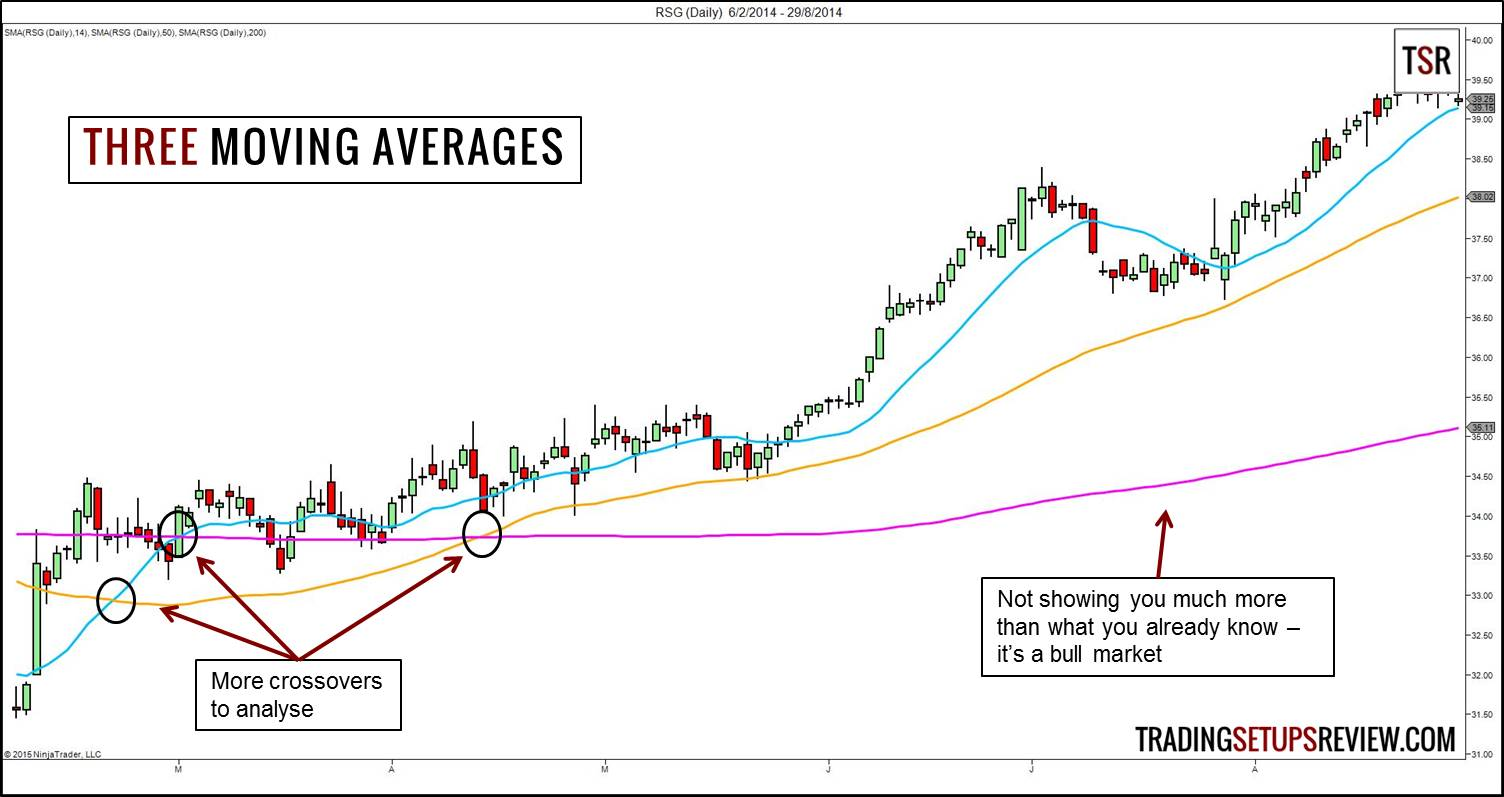
\includegraphics[width=1.0\textwidth]{img/multiple-technical-indicators.jpg}
\label{figure:multiple-technical-indicators}
\end{figure}

\section{Using Agents to Represent Traders in a Financial Market}
\label{section:using-agents-to-represent-traders-in-a-financial-market}

Using an agent-based model to represent a financial market is perhaps one of the
most natural ways to do so. The explanation for this is that any financial
market is, in fact, being constructed by a group of agents: the traders. In the
proposed method, agents follow the process depicted in Figure
\ref{figure:agent-architecture}.


\begin{figure}
\caption{Architecture of an agent} \centering
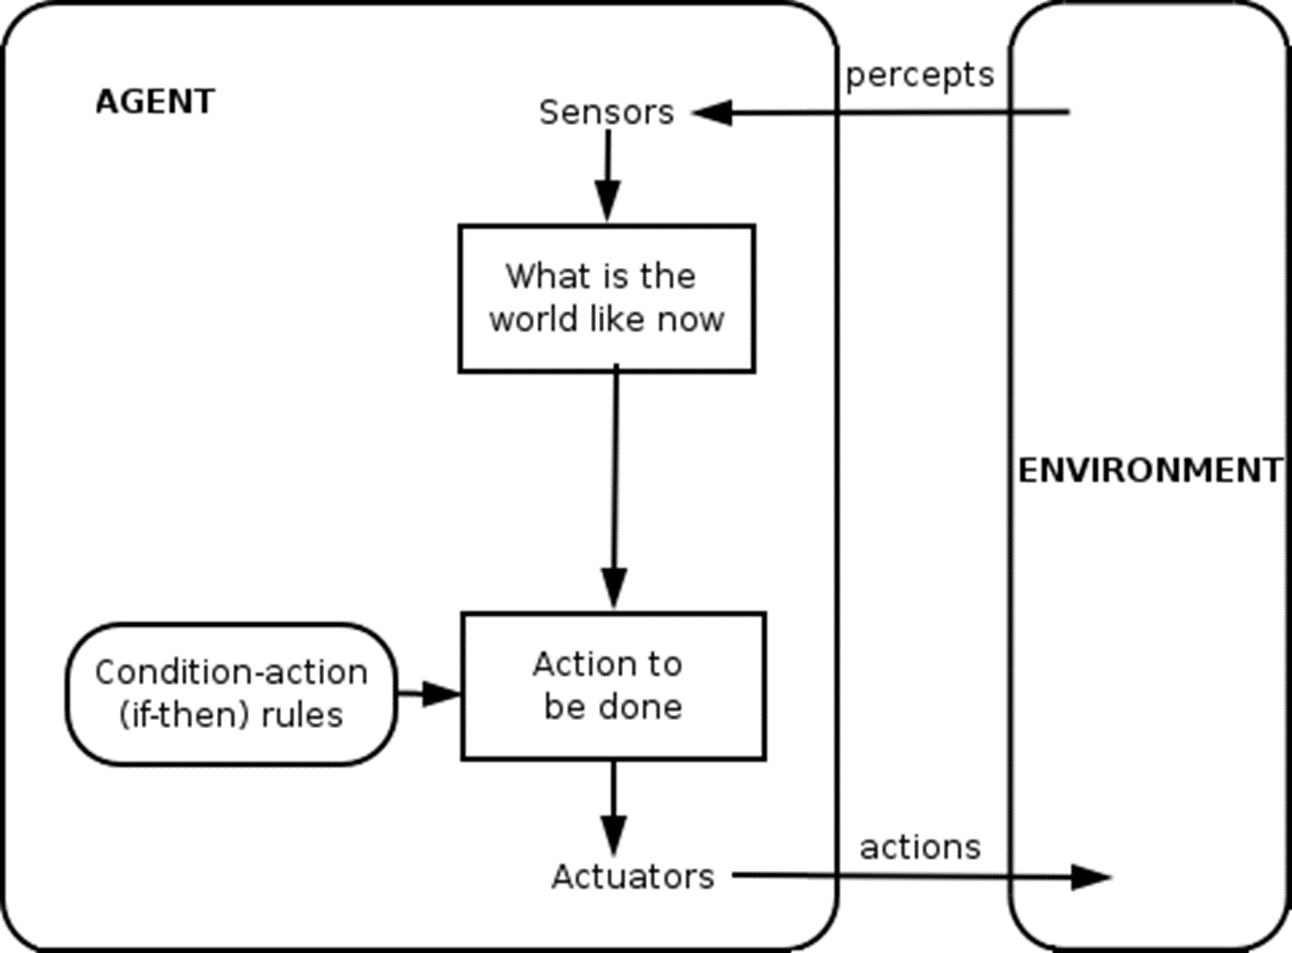
\includegraphics[width=1.0\textwidth]{img/agent-architecture.png}
\label{figure:agent-architecture}
\end{figure}

In this architecture, an agent is constantly sensing its environment, which, in
the case of this thesis, is the raw market prices coming from a broker. The
preprocessing mentioned in Section
\ref{section:preprocessing-a-financial-market-using-retracements} takes place as
part of each agent's sensing process; in other words, each agent has the
capability of preprocessing the market's raw data differently

\section{Using Retracements to Represent the Beliefs of a Trader}
\label{section:using-retracements-to-represent-the-beliefs-of-a-trader}

\section{Representing the Agents' Rules as Intuitionistic Fuzzy Systems}
\label{section:representing-the-agents-rules-as-intuitionistic-fuzzy-systems}

\subsection{Indeterminacy or Hesitancy}
\label{subsection:indeterminacy-or-hesitancy}

\section{Generation of an Agent-Based Model}
\label{section:generation-of-an-agent-based-model}

\section{Using the Agent-Based Model to Generate Insights about a Financial
Market}
\label{section:using-the-agent-based-model-to-generate-insights-about-a-financial-market}

\section{Using the Agent-Based Model to create a Trading Strategy}
\label{section:using-the-agent-based-model-to-create-a-trading-strategy}
